%%%%%%%%%%%%%%%%%%%%%%%%%%%%%%%%%%%%%%%%%%%%%%%%%%%%%%%%%%%%%%%%%%%%%%%%%%%%%
% 26/05/2010
% edited by Bill Lampos
%
% Feel free to use (copy) the structure (latex formatting source code)
% but not the content of this document.
%
%%%%%%%%%%%%%%%%%%%%%%%%%%%%%%%%%%%%%%%%%%%%%%%%%%%%%%%%%%%%%%%%%%%%%%%%%%%%%
\documentclass[compress,blue]{beamer}
\usepackage{etex}
\mode<presentation>

\usetheme{Warsaw}
% other themes: AnnArbor, Antibes, Bergen, Berkeley, Berlin, Boadilla, boxes, CambridgeUS, Copenhagen, Darmstadt, default, Dresden, Frankfurt, Goettingen,
% Hannover, Ilmenau, JuanLesPins, Luebeck, Madrid, Maloe, Marburg, Montpellier, PaloAlto, Pittsburg, Rochester, Singapore, Szeged, classic

%\usecolortheme{lily}
% color themes: albatross, beaver, beetle, crane, default, dolphin, dov, fly, lily, orchid, rose, seagull, seahorse, sidebartab, structure, whale, wolverine

%\usefonttheme{serif}
% font themes: default, professionalfonts, serif, structurebold, structureitalicserif, structuresmallcapsserif

% pdf is displayed in full screen mode automatically
%\hypersetup{pdfpagemode=FullScreen}

% define your own colours:
\definecolor{Red}{rgb}{1,0,0}
\definecolor{Blue}{rgb}{0,0,1}
\definecolor{Green}{rgb}{0,1,0}
\definecolor{magenta}{rgb}{1,0,.6}
\definecolor{lightblue}{rgb}{0,.5,1}
\definecolor{lightpurple}{rgb}{.6,.4,1}
\definecolor{gold}{rgb}{.6,.5,0}
\definecolor{orange}{rgb}{1,0.4,0}
\definecolor{hotpink}{rgb}{1,0,0.5}
\definecolor{newcolor2}{rgb}{.5,.3,.5}
\definecolor{newcolor}{rgb}{0,.3,1}
\definecolor{newcolor3}{rgb}{1,0,.35}
\definecolor{darkgreen1}{rgb}{0, .35, 0}
\definecolor{darkgreen}{rgb}{0, .6, 0}
\definecolor{darkred}{rgb}{.75,0,0}

\xdefinecolor{olive}{cmyk}{0.64,0,0.95,0.4}
\xdefinecolor{purpleish}{cmyk}{0.75,0.75,0,0}

% \usepackage{beamerinnertheme_______}
% inner themes include circles, default, inmargin, rectangles, rounded

%\usepackage{beamerouterthemesmoothbars}
% outer themes include default, infolines, miniframes, shadow, sidebar, smoothbars, smoothtree, split, tree

\useoutertheme[subsection=false]{smoothbars}

% to have the same footer on all slides
%\setbeamertemplate{footline}[text line]{xxx xxx xxx}
%\setbeamertemplate{footline}[text line]{} % or empty footer

% include packages
\usepackage{subfigure}
\usepackage{multicol}
\usepackage{amsmath}
\usepackage{epsfig}
\usepackage{helvet}
\usepackage{graphicx}
\usepackage[all,knot]{xy}
\xyoption{arc}
\usepackage{url}
\usepackage{multimedia}
\usepackage{hyperref}
\usepackage{setspace}
\usepackage{subfigure}

\title{Gradient Optimization}
\subtitle{Algorithms Comparison}
\author{Ali Saleh}
\date{\scriptsize Universit\"{a}t Hamburg \\ \vspace{.10cm}Jul 25, 2017}

\begin{document}

\frame{
	\titlepage
}

\section[Outline]{}
\frame{\tableofcontents}

\section{Introduction}
\subsection{What is a Gradient}
\frame{\frametitle{What is a Gradient}
  The gradient is a multi-variable generalization of the derivative
  \begin{figure}[hbtp]
    \centering
    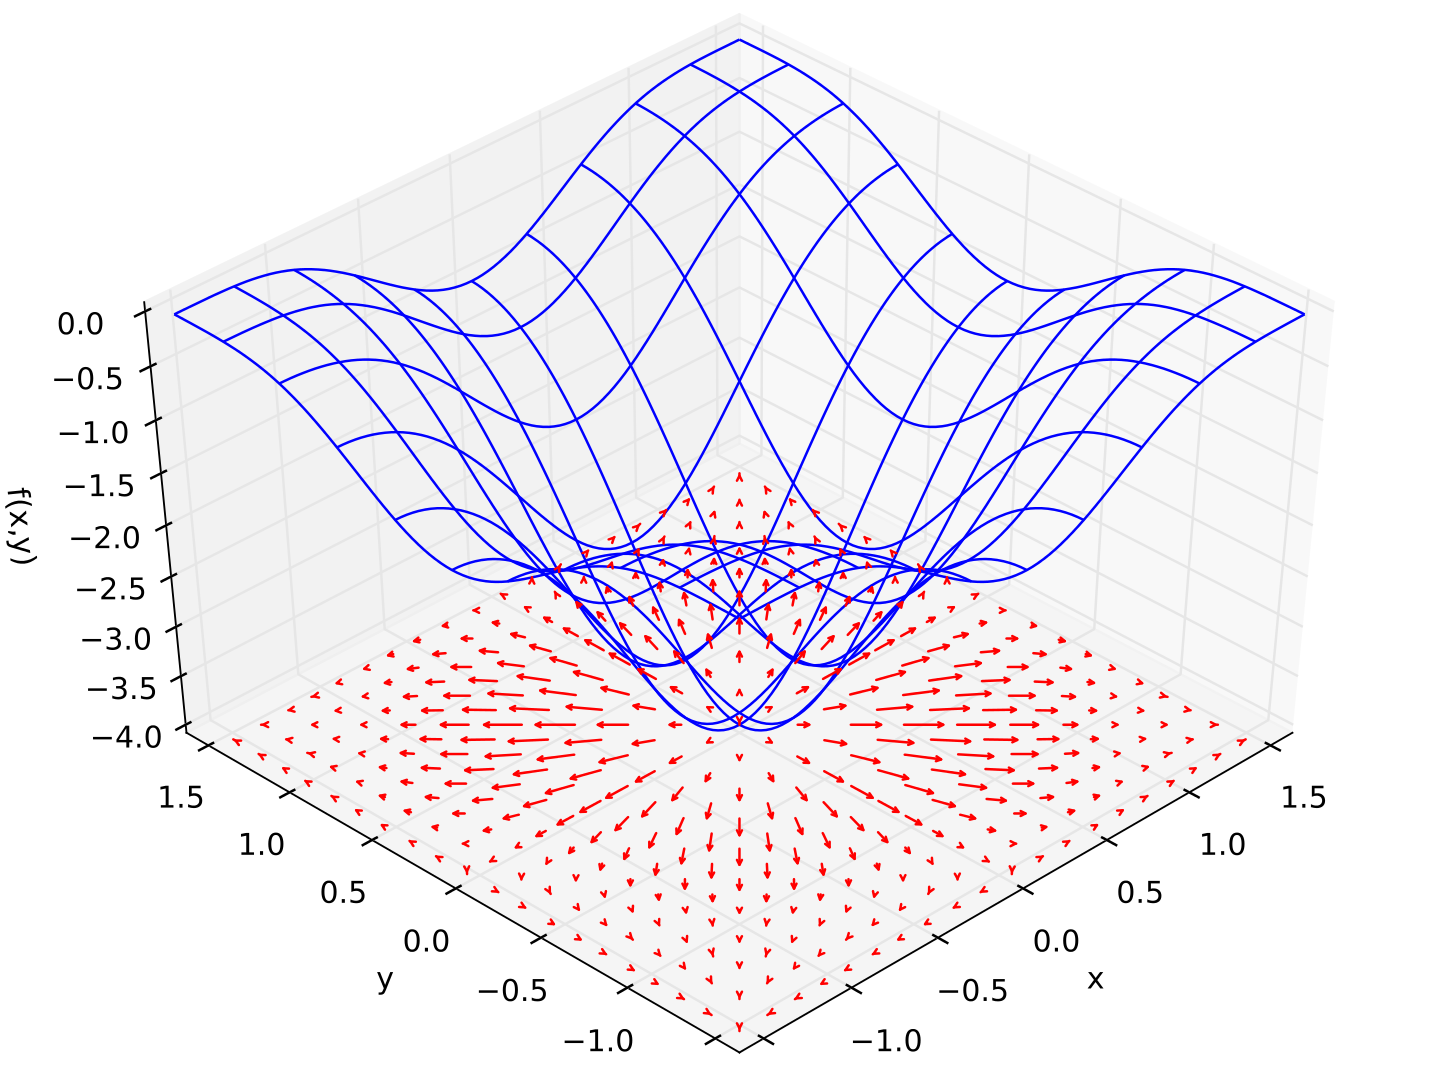
\includegraphics[width=190pt,height=160pt]{figures/Gradient_Visual.png}
    \caption{\scriptsize Gradient of a 2 Variable function projected as vector field [1]}
  \end{figure}
}

\subsection{Gradient in Neural Networks}
\frame{\frametitle{Gradient in Neural Networks}
  \begin{itemize}
  \item Used in minimizing model's objective function
  \item Parameters are updated in the opposite direction of objective function gradient
  \item The learning rate $\eta$ determines the size of the steps taken to reach minimum
  \end{itemize}

}

\section{Calculating The Gradient}
\subsection{Computing The Gradient}
\frame{\frametitle{Computing The Gradient}
  \begin{itemize}
  \item Using finite difference 
    \begin{enumerate}
    \item Calculate the partial derivative in each direction
    \item Slow and computationally expensive
    \end{enumerate}  
  \item Use calculus to find closed formulas for gradient
    \begin{enumerate}
    \item Gives faster results
    \item Open for method tweaking
    \item Can be harder to implement
    \end{enumerate}  
  \end{itemize}
}


\subsection{Basic Algorithms}
\frame{\frametitle{Basic Algorithms}
  \begin{itemize}
  \item Stochastic gradient descent (SGD)
    \begin{enumerate}
    \item Train a model
    \item Evaluate the gradient on a small batch of data
    \item Update the model parameters accordingly
    \item Slowly decreasing learning rate guarantee convergence
    \end{enumerate}  
  \item Momentum [2]
    \begin{enumerate}
    \item Use adaptive learning rate for different dimensions
    \end{enumerate}
  \end{itemize}
  \begin{figure}[hbtp]
    \centering
    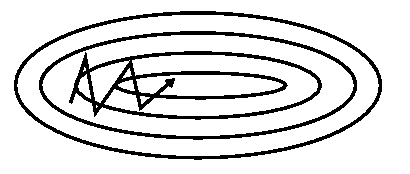
\includegraphics[width=60pt,height=40pt]{figures/with_momentum.png}
    \caption{\scriptsize SGD with momentum [3]}
  \end{figure}
}

\subsection{Adaptive Algorithms}
\frame{\frametitle{Adaptive Algorithms}
  \begin{itemize}
  \item Adagrad [4]
    \begin{enumerate}
    \item Use adaptive learning based on parameter update frequency
    \item Keeps a matrix of the squares of all past gradients
    \item Divide learning rate by the sum of all past square gradients
    \item Over time learning rate gets infinitesimally small
    \end{enumerate}
  \item Adam [5]
    \begin{enumerate}
    \item Use adaptive learning based on parameter update frequency
    \item Keeps track of the average of all past gradients
    \item Keeps track of the average of all past square of gradients
    \item Avoid the weakness of Adagrad
    \end{enumerate}
  \end{itemize}
  Both are more suitable for sparse datasets
}

\section{Experiment}
\subsection{Experiment Setup}
\frame{\frametitle{Experiment Setup}
\begin{itemize}
\item Build a convolution neural network using keras
\item Use 3 different optimization algorithms (SGD, Adam, Adagrad)
\item Optimize network parameters using hyperas (Keras + Hyperopt)
\item Use CIFAR10 dataset
\end{itemize}
}
b
\frame{\frametitle{CIFAR 10}
  \begin{figure}[hbtp]
    \centering
    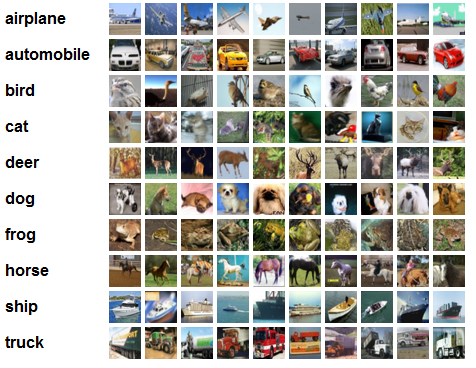
\includegraphics[width=200pt,height=160pt]{../Code/cifar_preview.png}
    \caption{overview of the CIFAR 10 dataset (courtesy of Alex Krizhevsky)}
  \end{figure}
}

\section{Results}
\subsection{Performance Metrics}
\frame{\frametitle{Time}
  \begin{figure}[H]
    \label{time}
    \centering
    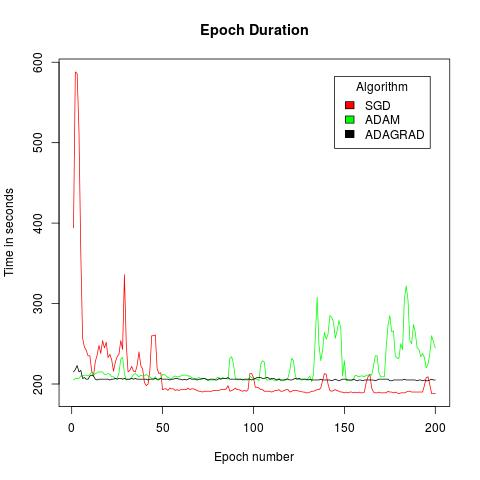
\includegraphics[scale=.35]{../Code/Time.jpg}
    \caption{Total execution time per epoch over time for each optimizer}
  \end{figure}
}

\frame{\frametitle{Loss}
  \begin{figure}[H]
    \centering
    \centering
    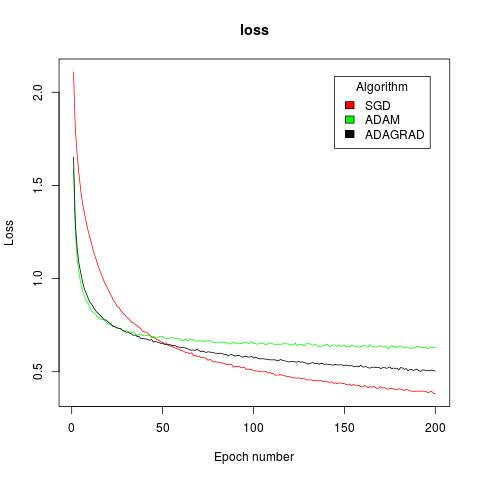
\includegraphics[scale=.35]{../Code/loss.jpg}
    \caption{Loss per epoch on test set}
  \end{figure}
  }

\frame{\frametitle{Validation Loss}
  \begin{figure}[H]
    \centering
    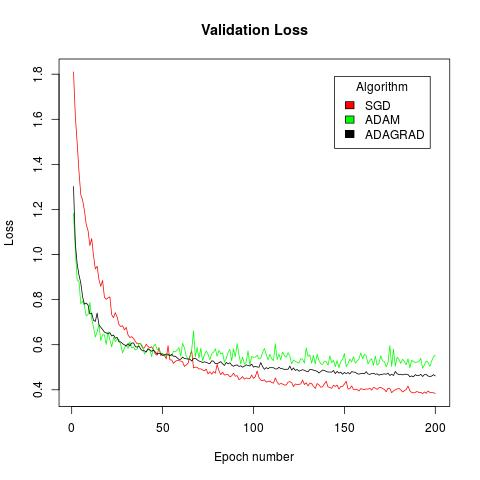
\includegraphics[scale=.35]{../Code/val_loss.jpg}
    \caption{Loss per epoch for on validation set}
  \end{figure}
}

\frame{\frametitle{Accuracy}
\begin{figure}[H]
  \centering
  \centering
  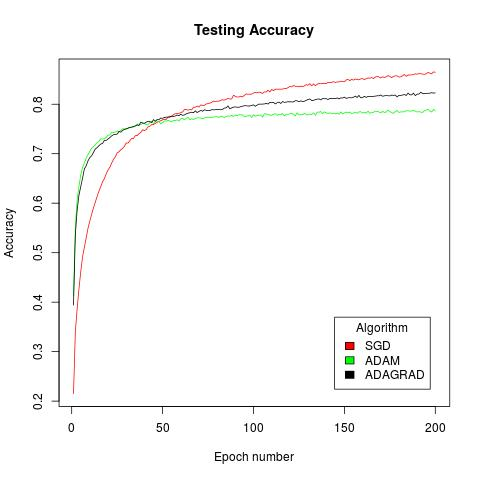
\includegraphics[scale=.35]{../Code/acc.jpg}
  \caption{Accuracy on test set}
\end{figure}
}

\frame{\frametitle{Validation Accuracy}
  \begin{figure}
    \centering
    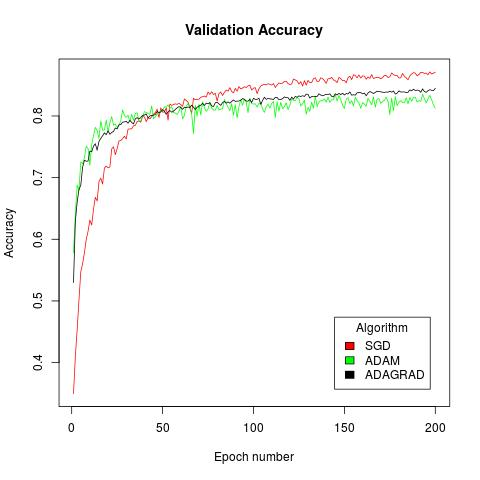
\includegraphics[scale=.35]{../Code/val_acc.jpg}
    \caption{Accuracy on validation set}
  \end{figure}
}

\subsection{General Statistics}
\frame{\frametitle{Statistics}
  \begin{table}[H]
    \scriptsize
    \centering % centering table
    \begin{tabular}{c r|r|r|r|r|r|} % creating eight columns
      \hline\hline %inserting double-line
      \multicolumn{1}{c}{} &\multicolumn{3}{c}{SGD} &\multicolumn{3}{c}{Adam}\\
      Metric & min& mean &max & min& mean &max\\
      \hline % inserts single-line
      Time & 188.0& 209.2 & 588.0& 203.0& 220.6& 322.0\\
      \hline
      Loss  & 0.3822 & 0.6041 & 2.1094& 0.6224& 0.6836& 1.5892\\
      \hline
      Accuracy & 0.2151 & 0.7865 & 0.8654& 0.4132& 0.7655& 0.7899\\
      \hline
      Validation Loss  & 0.3828 & 0.5363 & 1.8103& 0.4953& 0.5708& 1.1835\\
      \hline
      Validation Accuracy & 0.3496 & 0.8150 & 0.8715& 0.5782& 0.8075& 0.8353\\
      \hline % inserts single-line
    \end{tabular}
    \label{tab:hresult}
  \end{table}

  \begin{table}[H]
    \scriptsize
    \centering % centering table
    \begin{tabular}{c r|r|r} % creating eight columns
      \hline\hline %inserting double-line
      \multicolumn{1}{c}{} &\multicolumn{3}{c}{Adagrad}\\
      Metric & min& mean &max\\
      \hline % inserts single-line
      Time & 205.0& 206.1& 223.0 \\ % Entering row contents
      \hline
      Loss  &  0.5027& 0.6187& 1.6527 \\
      \hline
      Accuracy &  0.3942& 0.7827& 0.8242 \\
      \hline
      Validation Loss  &  0.4577& 0.5391& 1.3018 \\
      \hline
      Validation Loss &  0.5298& 0.8131& 0.8449 \\
      \hline % inserts single-line
    \end{tabular}
    \label{tab:hresult}
  \end{table}
}

\section*{}
\frame{
    \begin{center}
        \huge
        This is the last slide.\\ 
        \vspace{1cm}
        Any questions?
    \end{center}
}

\frame{\frametitle{References}
\begin{enumerate}
\item https://en.wikipedia.org/wiki/Gradient
\item Qian, N. (1999). On the momentum term in gradient descent learning algorithms. Neural Networks : The Official Journal of the International Neural Network Society
\item http://ruder.io/optimizing-gradient-descent/index.html
\item Zeiler, M. D. (2012). ADADELTA: An Adaptive Learning Rate Method
\item Kingma, D. P., & Ba, J. L. (2015). Adam: a Method for Stochastic Optimization. International Conference on Learning Representations,
\end{enumerate}
}
\end{document} 
